\documentclass{article}
\usepackage[margin=1in]{geometry}
\usepackage{amsmath}
\usepackage{amssymb}
\usepackage{amsthm}
\usepackage{bm}
\usepackage{hyperref}
\usepackage{graphicx}
\usepackage{caption}
\usepackage{listings}
\usepackage{xcolor}
\usepackage{float}
\usepackage{booktabs}
\usepackage{longtable}
\usepackage{multirow}
\usepackage{placeins}
\graphicspath{{figures/}}

% Code style
\lstdefinestyle{code}{
  basicstyle=\ttfamily\small,
  numbers=left,
  numberstyle=\tiny,
  numbersep=8pt,
  keywordstyle=\color{blue},
  commentstyle=\color{teal!70!black},
  stringstyle=\color{orange!70!black},
  showstringspaces=false,
  breaklines=true,
  frame=single,
  framerule=0.3pt,
  rulecolor=\color{black!15}
}
\lstset{style=code}

\title{Training Frameworks in Practice: Transformers, Distributed Engines, Checkpoints, and Monitoring}
\author{}
\date{\today}

\begin{document}
\maketitle

\section{End-to-End Hugging Face Transformers Pipeline}
\subsection{Workflow overview}
The Hugging Face ecosystem offers a modular loop from dataset curation through evaluation and registry publishing. Figure~\ref{fig:hf_pipeline_en_tf} summarizes the canonical flow, highlighting how datasets, tokenization, training arguments, accelerator plugins, and artifact management fit together.
\begin{figure}[H]
  \centering
  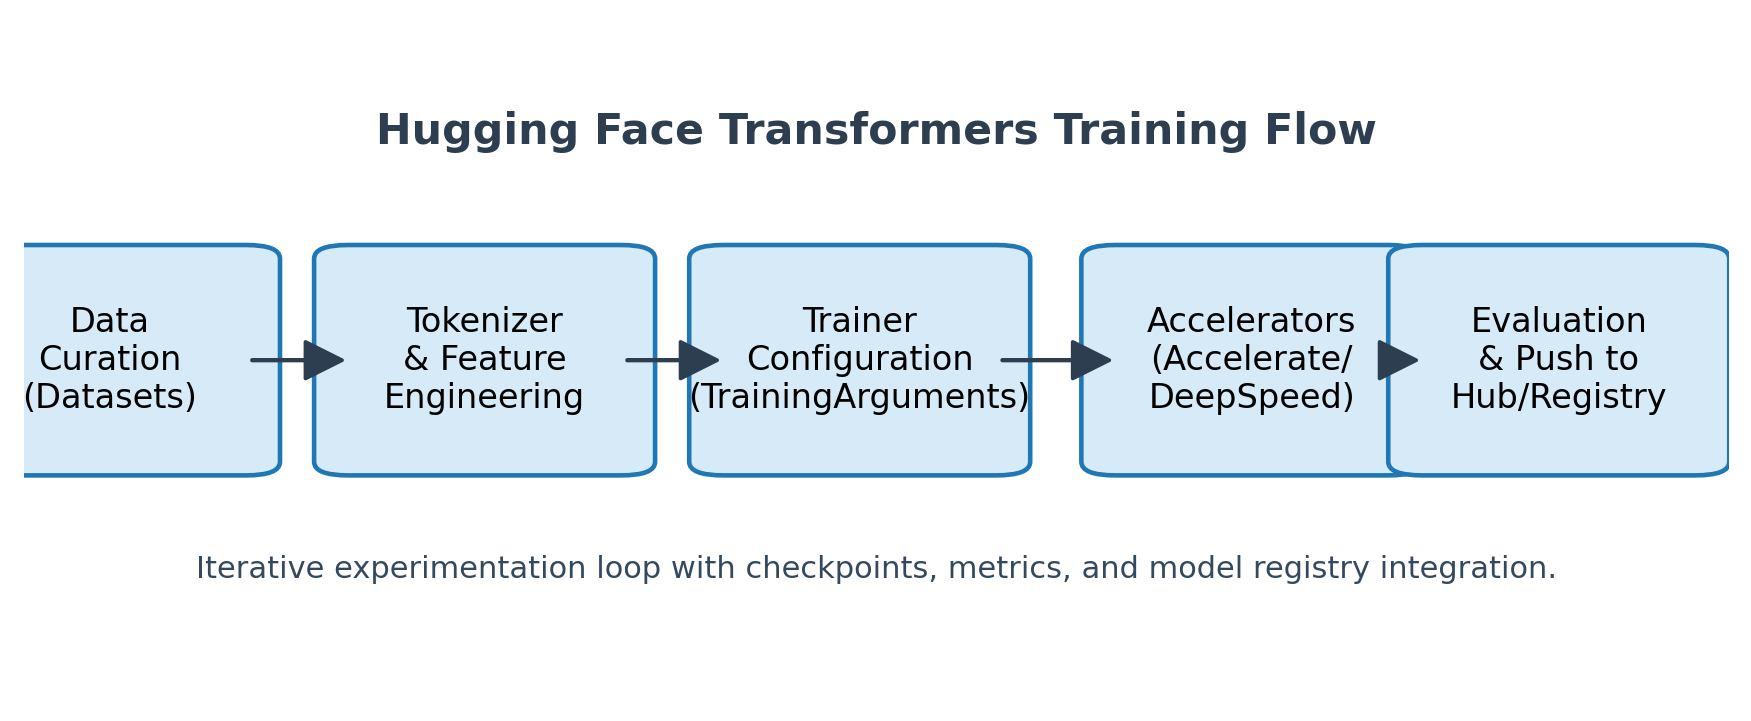
\includegraphics[width=0.9\textwidth]{hf_training_pipeline.png}
  \caption{Hugging Face Transformers pipeline: dataset preparation, feature engineering, training configuration, accelerator integration, and model delivery.}
  \label{fig:hf_pipeline_en_tf}
\end{figure}
Key stages:
\begin{enumerate}
  \item \textbf{Dataset ingestion:} Leverage the \texttt{datasets} library for local or remote loading, streaming, schema inference, and map/filter transforms. Combine with fast tokenizers for truncation, dynamic padding, and special-token handling.
  \item \textbf{Model selection:} \texttt{AutoModelForCausalLM}, \texttt{AutoModelForSeq2SeqLM}, and \texttt{AutoConfig} provide architecture-specific defaults while exposing knobs for hidden sizes, attention heads, cache length, and parallelization.
  \item \textbf{Trainer orchestration:} \texttt{Trainer} plus \texttt{TrainingArguments} deliver gradient accumulation, LR schedulers, mixed precision (fp16/bf16), logging hooks, and multi-accelerator support. Callbacks allow early stopping, metric-based checkpointing, or custom artifact uploads.
  \item \textbf{Evaluation and release:} Evaluate via \texttt{Trainer.evaluate} or custom loops, integrate with \texttt{evaluate} metrics, and serialize the bundle (model, tokenizer, config, adapter weights) for Hugging Face Hub or internal registries.
\end{enumerate}

\subsection{Efficiency levers}
\begin{itemize}
  \item \textbf{Input pipeline:} Streaming datasets paired with dynamic padding collators prevent idle GPU cycles; for TPU pods, shard iterables and cache vocabulary locally.
  \item \textbf{Precision and compilation:} Use bf16 on A100/H100 for numerical stability; combine \texttt{torch.compile}, FlashAttention, or DeepSpeed ZeRO for extra throughput.
  \item \textbf{Parameter-efficient tuning:} Integrate LoRA/QLoRA/Adapters via the \texttt{peft} stack to cut memory costs while keeping high-quality adaptation.
  \item \textbf{Experiment automation:} Manage runs through \texttt{HfArgumentParser} + YAML configs; log metrics, gradients, and checkpoints with W\&B or MLflow for reproducibility.
\end{itemize}

\subsection{Reference template}
\begin{lstlisting}[language=Python,caption={Instruction tuning with Hugging Face Trainer}]
from datasets import load_dataset
from transformers import (
    AutoTokenizer,
    AutoModelForCausalLM,
    TrainingArguments,
    Trainer,
    DataCollatorForLanguageModeling,
)

model_name = "mistralai/Mistral-7B-Instruct-v0.3"
tokenizer = AutoTokenizer.from_pretrained(model_name, use_fast=True)
dataset = load_dataset("json", data_files={"train": "train.jsonl", "eval": "eval.jsonl"})

def preprocess(batch):
    return tokenizer(batch["prompt"], text_target=batch["answer"], truncation=True)

tokenized = dataset.map(preprocess, batched=True, remove_columns=dataset["train"].column_names)
collator = DataCollatorForLanguageModeling(tokenizer, mlm=False)
model = AutoModelForCausalLM.from_pretrained(model_name, torch_dtype="bfloat16")

args = TrainingArguments(
    output_dir="outputs/mistral-instruct",
    per_device_train_batch_size=4,
    gradient_accumulation_steps=8,
    num_train_epochs=2,
    learning_rate=2e-5,
    logging_steps=20,
    evaluation_strategy="steps",
    eval_steps=400,
    save_steps=400,
    bf16=True,
    report_to=["wandb"],
    push_to_hub=True,
)

trainer = Trainer(
    model=model,
    args=args,
    train_dataset=tokenized["train"],
    eval_dataset=tokenized["eval"],
    data_collator=collator,
)

trainer.train()
\end{lstlisting}

\section{DeepSpeed, Megatron-LM, and ColossalAI}
\subsection{Capability landscape}
Three leading frameworks target trillion-scale training through complementary parallelism strategies. Figure~\ref{fig:distributed_landscape_en_tf} compares their strengths.
\begin{figure}[H]
  \centering
  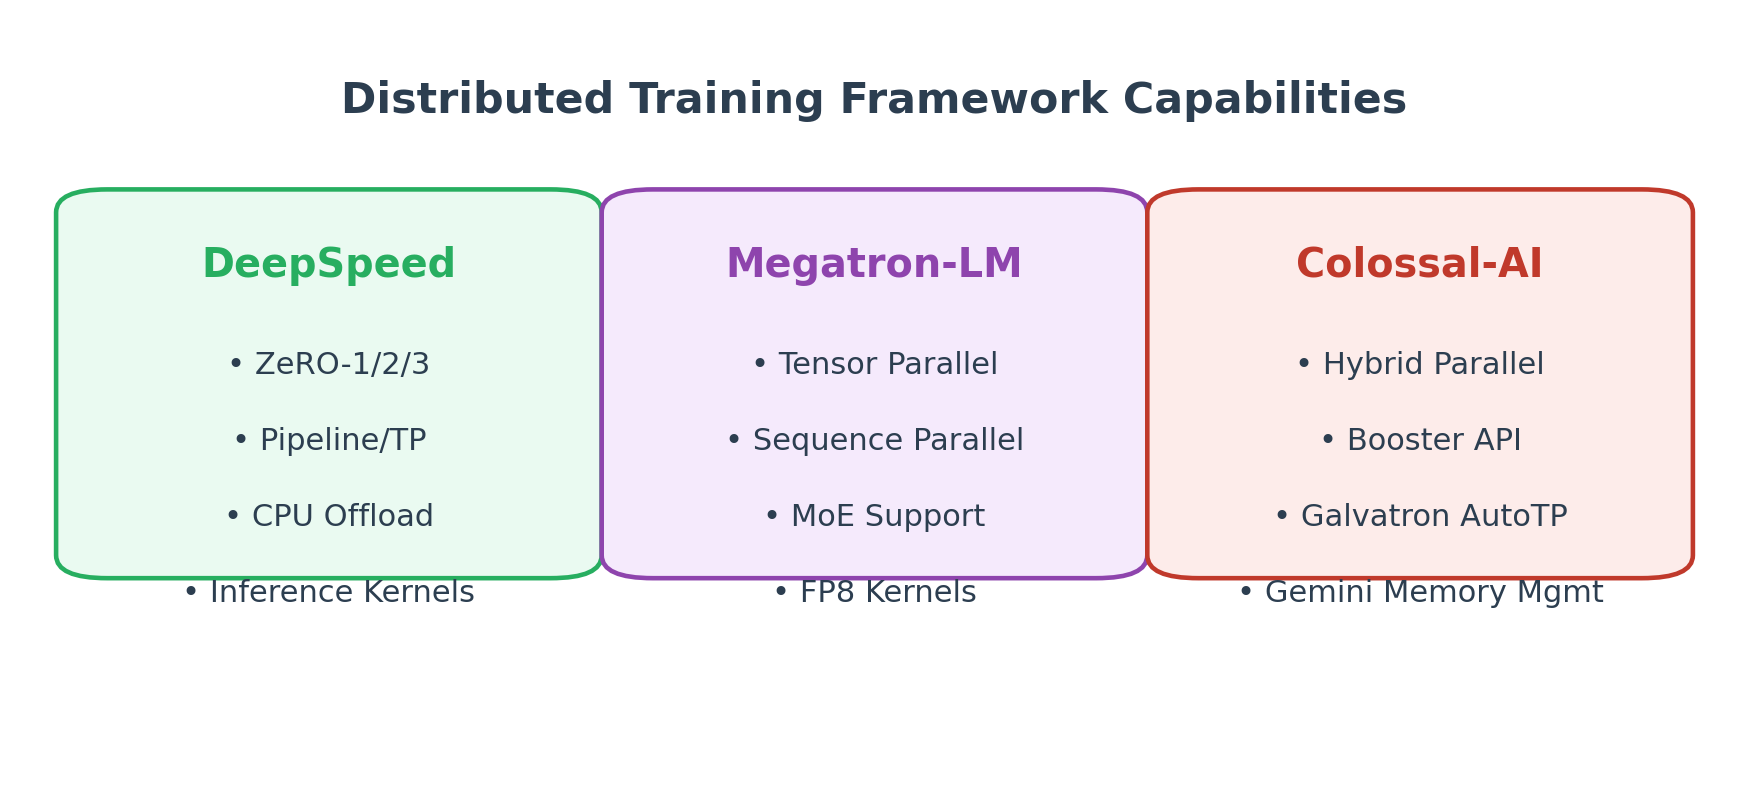
\includegraphics[width=0.9\textwidth]{distributed_frameworks.png}
  \caption{Distributed training framework capabilities.}
  \label{fig:distributed_landscape_en_tf}
\end{figure}
\begin{longtable}{p{3.2cm}p{5cm}p{6cm}}
\toprule
Framework & Highlights & Best fit \\
\midrule
DeepSpeed & ZeRO-1/2/3, ZeRO-Offload, inference optimizations, compression tooling & Autoregressive models spanning dozens of GPUs with memory fragmentation constraints \\
Megatron-LM & Tensor/sequence parallelism, pipeline parallel, MoE, FP8 kernels & GPT/MoE pretraining on dense GPU clusters with deterministic reproducibility \\
ColossalAI & Hybrid parallel, Gemini memory management, Booster API, Galvatron auto tensor-parallel search & Research/enterprise stacks requiring flexibility, auto-parallel tuning, and memory-aware dispatch \\
\bottomrule
\end{longtable}

\subsection{ZeRO and hybrid parallelism}
ZeRO partitions optimizer states, gradients, and parameters to remove redundancy:
\begin{itemize}
  \item \textbf{Stage 1:} Shard optimizer state (e.g., Adam moments) across data-parallel ranks.
  \item \textbf{Stage 2:} Shard gradients as well, lowering all-reduce payloads.
  \item \textbf{Stage 3:} Partition parameters, broadcasting slices on demand and enabling 100B+ models.
\end{itemize}
Combine ZeRO with pipeline and tensor parallelism to construct hybrid strategies that match cluster topology and model architecture.

\subsection{Operational practices}
\begin{itemize}
  \item \textbf{Planning order:} Fix ZeRO stage first, then choose tensor parallel degree (aligned with head counts or MLP factorization), and finally determine pipeline cuts to balance micro-batches.
  \item \textbf{Communication:} Optimize NCCL topology (NVSwitch/NVLink/InfiniBand), enable overlap of compute and communication, and experiment with compressed gradient schemes (1-bit Adam, PowerSGD).
  \item \textbf{Fault tolerance:} DeepSpeed checkpointing, Megatron tensor-parallel recovery, and ColossalAI Gemini snapshots mitigate node failures.
  \item \textbf{Mixture-of-experts:} Tune top-$k$ routing, capacity factor, and load-balancing loss; allocate expert parallel ranks carefully to avoid hotspots.
\end{itemize}

\section{Checkpoint Merging, Conversion, and Pruning}
\subsection{Common scenarios}
Large-scale training generates diverse checkpoints requiring downstream processing:
\begin{itemize}
  \item \textbf{Merge adapters:} Fold LoRA adapters into base weights for inference deployment.
  \item \textbf{Combine shards:} Reconstruct single-rank weights from tensor-parallel shards or ZeRO partitions.
  \item \textbf{Format conversions:} Transform PyTorch safetensors into GGUF, TensorRT/ONNX engines, or custom runtime bundles.
  \item \textbf{Structural pruning:} Trim position embeddings, drop unused adapters, or clip maximum sequence lengths for efficiency.
\end{itemize}

\subsection{Tools and pipelines}
\begin{longtable}{p{3.2cm}p{4cm}p{6cm}}
\toprule
Tool & Function & Notes \\
\midrule
\texttt{peft.merge\_lora.py} & Merge LoRA adapters & Export as safetensors to avoid FP16 rounding issues \\
\texttt{transformers.convert} utilities & Cross-architecture conversion (BLOOM, OPT, GPT-NeoX) & Ensure vocab/tokenizer alignment and target shard sizes \\
llama.cpp scripts & Produce GGUF/GGML quantized weights & Quantize post-merge, then verify perplexity regression \\
TensorRT-LLM \texttt{trtllm-build} & Compile FP16/INT8 engines with KV planner & Provide calibration sets and match runtime scheduler settings \\
\bottomrule
\end{longtable}

\subsection{Example: merge LoRA and export ONNX}
\begin{lstlisting}[language=Python,caption={Consolidating LoRA adapters and exporting to ONNX}]
from transformers import AutoModelForCausalLM, AutoTokenizer
from peft import PeftModel
import torch

base = "Qwen/Qwen2-7B"
lora_dir = "outputs/qwen2-lora"
target_dir = "artifacts/qwen2-export"

tokenizer = AutoTokenizer.from_pretrained(base)
model = AutoModelForCausalLM.from_pretrained(base, torch_dtype=torch.float16)
model = PeftModel.from_pretrained(model, lora_dir)
model = model.merge_and_unload()
model.save_pretrained(target_dir, safe_serialization=True)
tokenizer.save_pretrained(target_dir)

dummy = torch.randint(0, tokenizer.vocab_size, (1, 256), dtype=torch.long)
torch.onnx.export(
    model,
    (dummy,),
    f"{target_dir}/model.onnx",
    input_names=["input_ids"],
    output_names=["logits"],
    dynamic_axes={"input_ids": {0: "batch", 1: "sequence"}},
    opset_version=18,
)
\end{lstlisting}
Always validate export correctness with ONNX Runtime or TensorRT inference, checking numerical parity against the reference PyTorch model.

\section{Distributed Training and Monitoring (W\&B, TensorBoard)}
\subsection{Metric design}
Robust monitoring extends beyond loss curves:
\begin{itemize}
  \item \textbf{System metrics:} GPU/CPU utilization, memory footprint, NIC throughput, disk I/O.
  \item \textbf{Training metrics:} Loss, perplexity, gradient norms, learning rate, gradient clipping ratios.
  \item \textbf{Communication:} AllReduce times, ZeRO synchronization latency, parameter staleness.
  \item \textbf{Quality:} Validation metrics, BLEU/ROUGE/BERTScore, human preference ratings, safety classifiers.
\end{itemize}

\subsection{Weights \& Biases integration}
W\&B provides experiment tracking, artifacts, and sweeps:
\begin{itemize}
  \item Log scalars, histograms, and text/audio samples via \texttt{wandb.log} or Trainer callbacks.
  \item Promote checkpoints to W\&B Artifacts for lineage tracking and promotion workflows.
  \item Launch sweeps for automated hyperparameter searches, orchestrating with Ray Tune or internal schedulers.
  \item Configure environment variables (\texttt{WANDB\_START\_METHOD=thread}) to avoid fork conflicts in multi-GPU setups.
\end{itemize}

\subsection{TensorBoard and custom visualization}
TensorBoard remains a reliable option for infrastructure-constrained teams:
\begin{itemize}
  \item Use \texttt{SummaryWriter} to log scalars, histograms, graphs, and embeddings.
  \item Restrict writes to rank 0 or aggregate logs manually to avoid contention.
  \item Export embeddings for projector visualizations to debug representation drift.
  \item Enable the profiler plugin to capture kernel timings, memory transfers, and communication traces.
\end{itemize}

\subsection{Alerting and automation}
Monitoring should trigger action when anomalies appear:
\begin{itemize}
  \item Forward metrics to Prometheus/Grafana; define alerts for OOM, NaN loss, or degraded throughput.
  \item Integrate Slack/Webhook notifications via W\&B alerts or custom scripts.
  \item Implement automated remediation scripts—e.g., reduce batch size, downgrade ZeRO stage, or pause training when health checks fail.
  \item Version-control experiment metadata (hyperparameters, git commit, dataset hash) for auditability.
\end{itemize}

\section*{Operational guidance}
\begin{itemize}
  \item Establish reusable configuration templates and shell/python launchers to standardize data prep, training, evaluation, and export.
  \item Validate distributed frameworks with minimal repro scripts before scaling out; document NCCL, topology, and environment variables.
  \item Pair checkpoint manipulations with parity checks (hashes, perplexity, functional tests) prior to deployment.
  \item Consolidate monitoring artifacts with experiment metadata for efficient root-cause analysis later.
\end{itemize}

\section*{Further reading}
\begin{itemize}
  \item Rajbhandari et al. ``ZeRO: Memory Optimizations Toward Training Trillion Parameter Models.'' SC, 2020.
  \item Narayanan et al. ``Efficient Large-Scale Language Model Training on GPU Clusters Using Megatron-LM.'' NeurIPS, 2021.
  \item Jiang et al. ``Colossal-AI: A Unified Deep Learning System For Large-Scale Parallel Training.'' arXiv, 2022.
  \item Hugging Face. ``Transformers Documentation.'' 2024.
  \item Biewald. ``Experiment Tracking with Weights and Biases.'' ODSC, 2020.
\end{itemize}

\end{document}

